\chapter{Algorithm}\label{cp:algo}

This chapter explains the general principles behind the algorithm and separates the logic from the implementation, which will be discussed in a separate chapter, \nameref{cp:sw}. 

The top plot in figure \ref{fig:algoOverview} shows one data set and how it is divided into different steps for processing. The first part (green) is when the user pumps up the cuff pressure. The second part (blue) is the deflation. Here, the oscillations are recorded and analysed as shown in the bottom plot. Once these oscillations have increased and decreased again to a certain value, the last step (red) is simply the deflation of the cuff. 


\begin{figure}[ht]
\centering
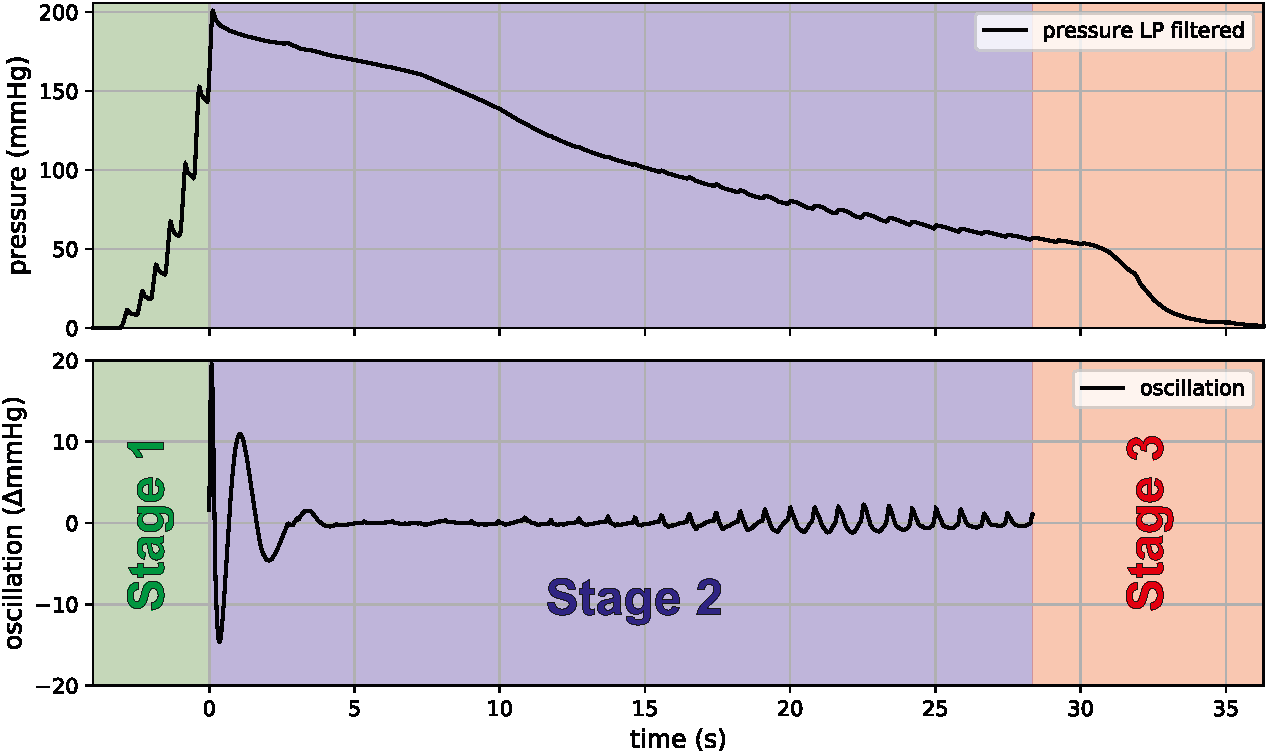
\includegraphics[width=\textwidth]{figures/algo_overview.pdf}
\caption{A sample data set is shown in the top plot and divided into three parts. The blue part is where oscillations are analysed. These are shown in the bottom plot.}
\label{fig:algoOverview}
\end{figure}


\section{Preprocessing}
The data is always filtered. Additionally, the first stage detects if the pressure is high enough to start the deflation process and therefore start feeding the data to the algorithm. Only the deflating and filtered data is processed by the core algorithm. 

\subsection{Filtering}
To remove unwanted noise from the data and to get the oscillations, two filters are used. Figure \ref{fig:stage1} shows the simple cascade of a low-pass (LP) and high-pass (HP) filter, resulting in a bandpass filtered output signal, the oscillogram. The results of both filter outputs are used in the algorithm.
%
%\begin{figure}[ht]
%\centering
%\includegraphics[width=0.7\textwidth]{figures/filter_cascade.pdf}
%\caption{The simple basic data processing flow. The data is acquired and passed first to a low-pass filter \SI{10}{\Hz} and then to a high-pass filter of \SI{0.5}{\Hz}, resulting in a bandpass output.}
%\label{fig:filter_cascade}
%\end{figure}

From the research done in chapter \ref{cp:theory}, it is known that most algorithms use band pass filters of low orders up to \ngith{6} and with cut-off frequencies between \SIrange{0.1}{0.5}{\Hz} and \SIrange{5}{20}{\Hz} \citep{Forouzanfar2015}. The implemented algorithm does not rely on pulse shape and can therefore use relaxed constraints. Best results were achieved with a lower cut-off frequency of \SI{0.5}{\Hz}. The upper cut-off frequency was fixed \SI{10}{\Hz}. Generally, there is very little activity between \SIrange{5}{20}{\Hz}, but because no experiments could be made, a mean value was chosen. 

\begin{figure}[ht]
\centering
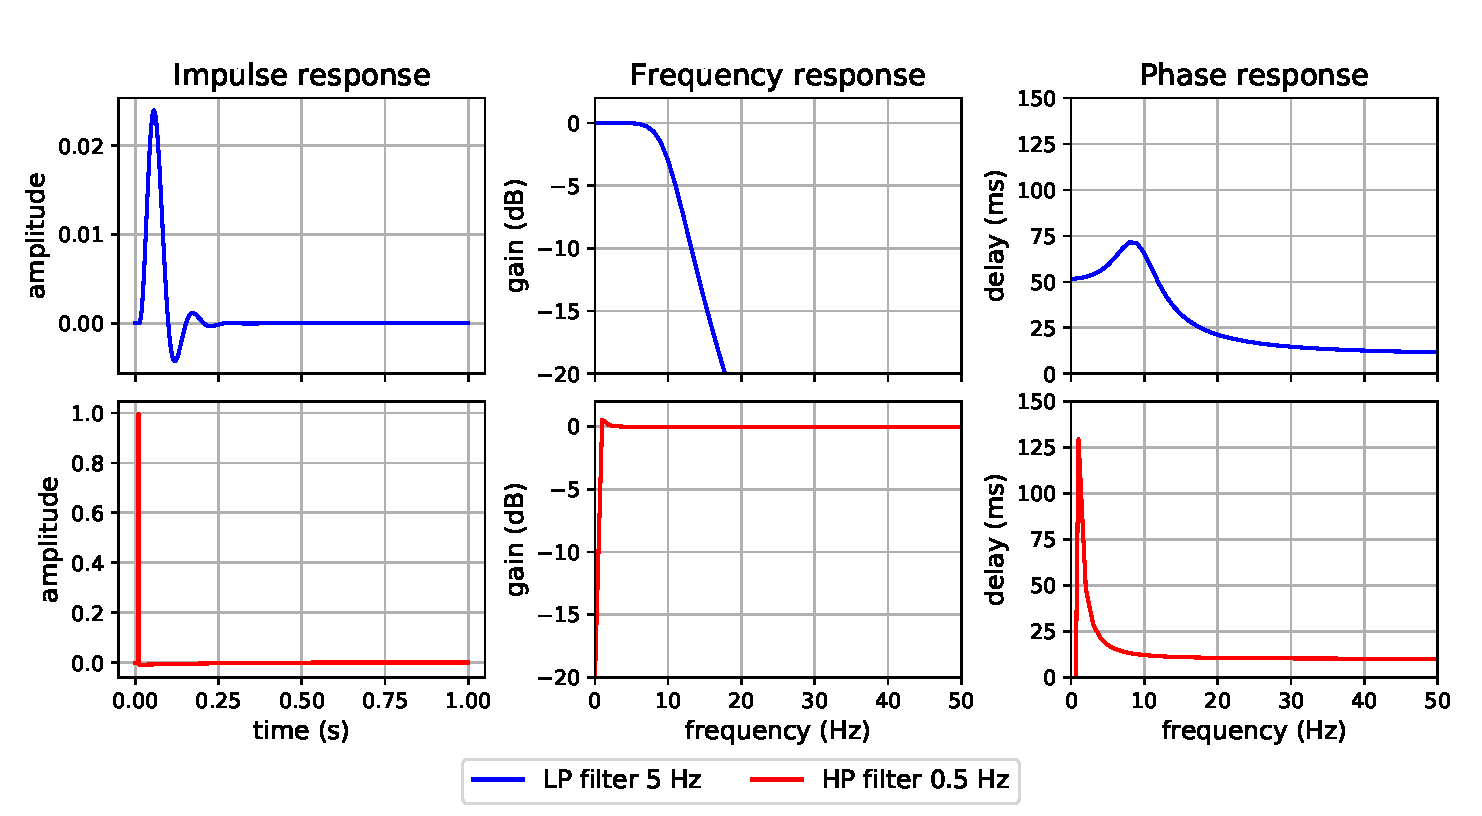
\includegraphics[width=\textwidth]{figures/filter.pdf}
\caption{Filter.}
\label{fig:filters}
\end{figure}
%All data is filtered. 
The implemented filters are shown in figure \ref{fig:filters}. The low-pass filter has a small delay in the impulse response and the phase response shows that for very low frequencies there is a slightly higher delay. The frequency response shows a steep slope after \SI{10}{\Hz} and suppression of more than \SI{20}{\decibel} of every frequency above \SI{20}{\Hz}. The HP filter expectedly lets the impulse pass. In the frequency response there is a small overshoot but otherwise a good suppression of DC. The bottom left plot in figure \ref{fig:filters} shows that HP filter has a significantly higher delay for frequencies around \SI{1}{\Hz}, of about \SI{125}{\milli\second}. This could potentially cause inaccuracies. Section \ref{fig:algoDetail} will show, why this is not a problem.


%TODO referecne section


\subsection{Inflation Detection}
The first stage of the data processing only checks, if the pressure in the cuff is high enough to start the deflation, which is the second stage.

\begin{figure}[ht]
\centering
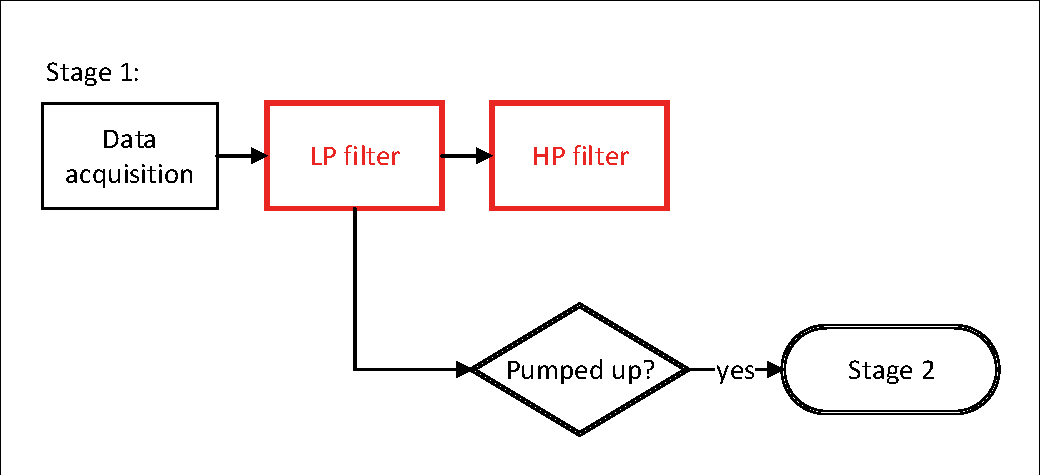
\includegraphics[width=0.7\textwidth]{figures/stage1.pdf}
\caption{The simple basic data processing flow. The data is acquired and passed first to a low-pass filter (\SI{10}{\Hz}) and then to a high-pass filter (\SI{0.5}{\Hz}), resulting in a bandpass output. The first stage of the data processing only checks, if the pressure in the cuff is high enough to start deflation (stage 2).}
\label{fig:stage1}
\end{figure}

\section{Deflation}
explain graph

\begin{figure}[ht]
\centering
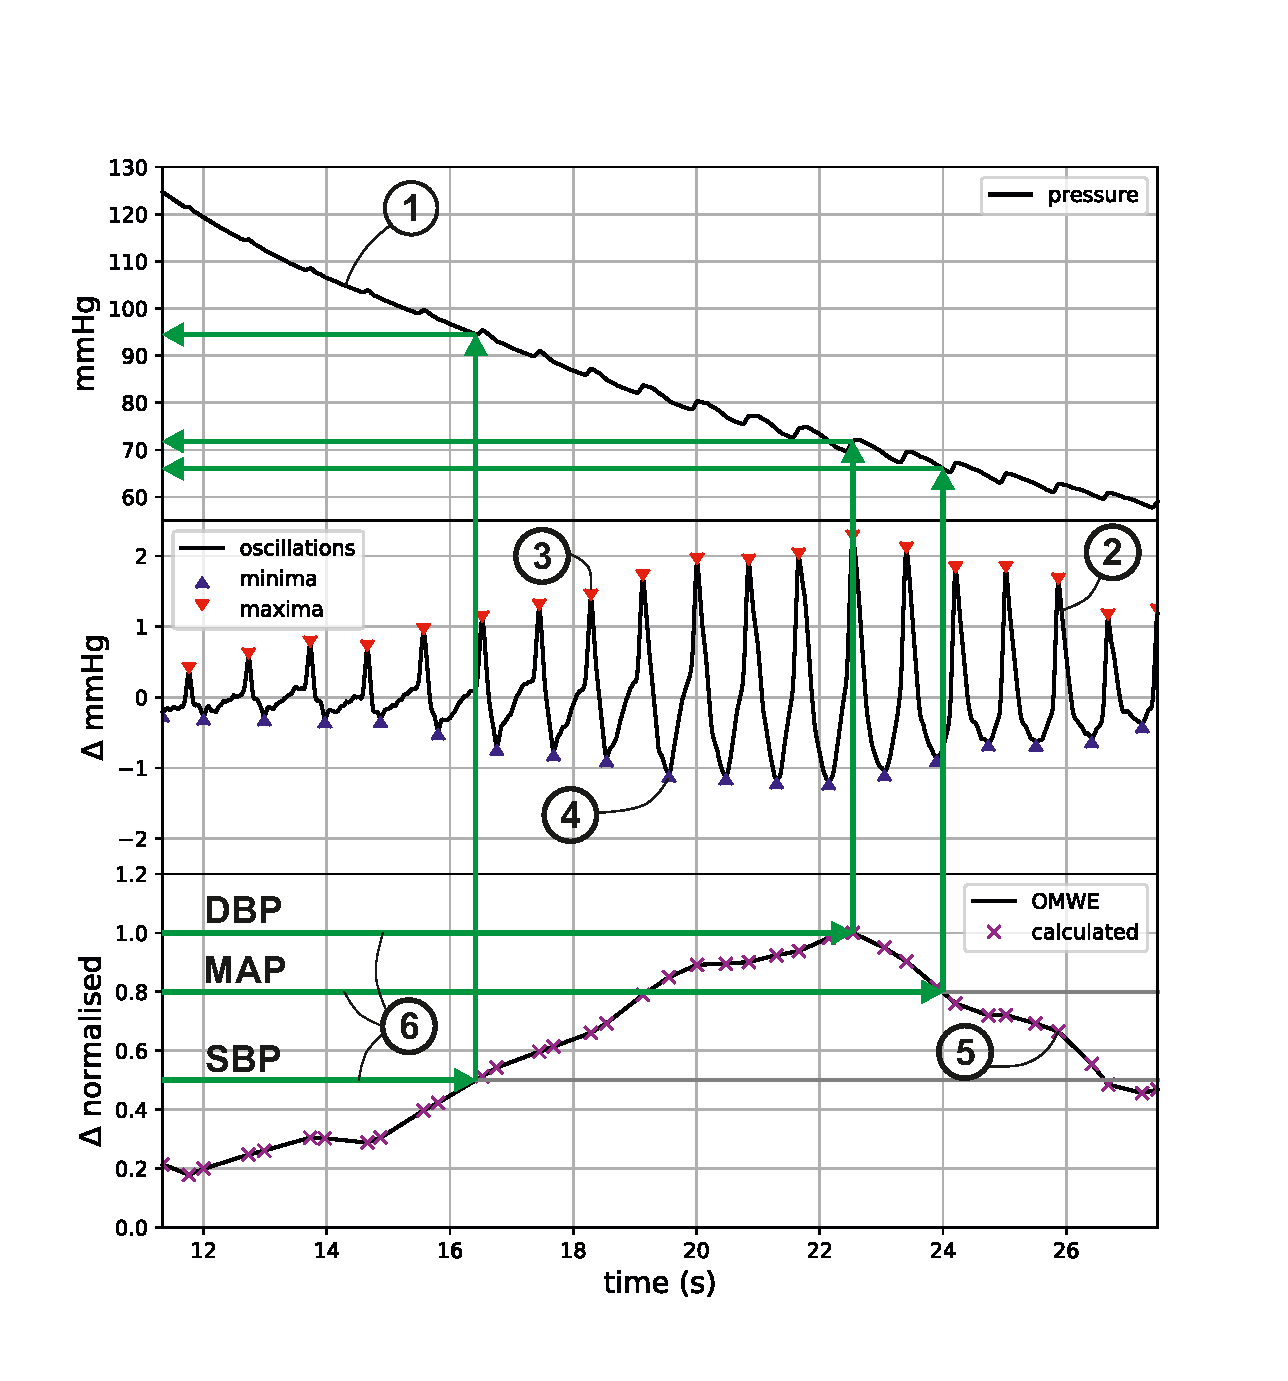
\includegraphics[width=\textwidth]{figures/algorithm_example_annotated.pdf}
\caption{Algo explanation.}
\label{fig:algoExplain}
\end{figure}



\begin{figure}[ht]
\centering
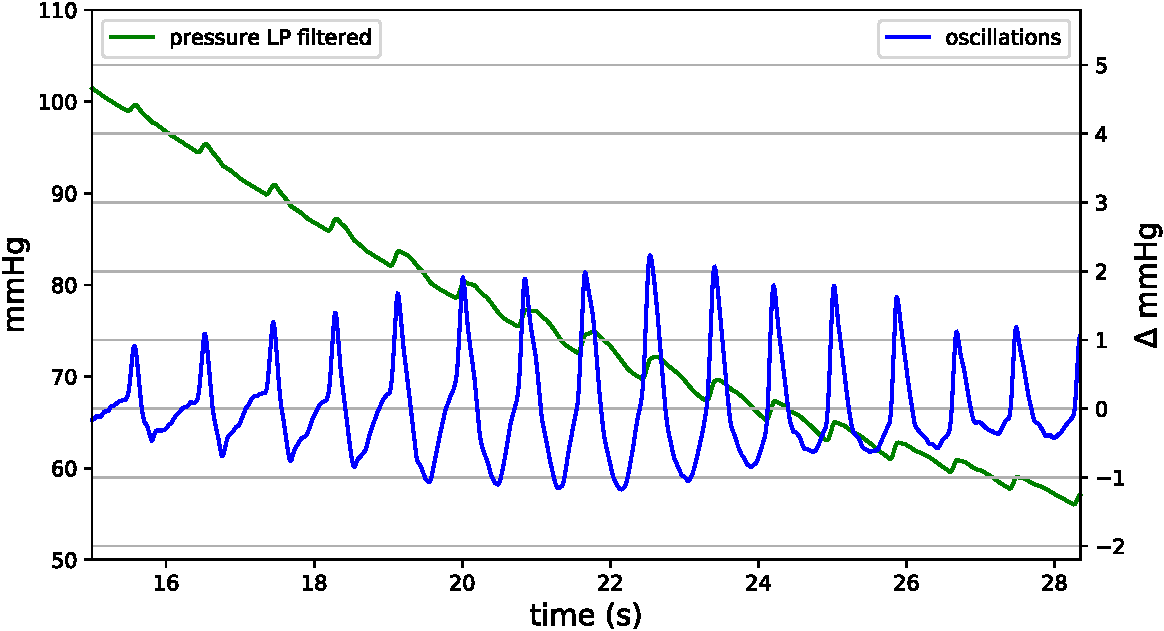
\includegraphics[width=\textwidth]{figures/algo_detail.pdf}
\caption{Algo explanation.}
\label{fig:algoDetail}
\end{figure}
\subsection{Extrema Detection}
minima
maxima

\subsection{Heart Rate Detection}
calculation of momentary heart beat from last two maxima



\section{Oscillometric Wave Envelope}
Interpolation between extrema to calculate Oscillometric Wave Envelope (OMWE).

\subsection{Determination of MAP, SBP and DBP}
check oscillation time in pressure, average over heart rate period.
\subsubsection{MAP}
max value
\subsubsection{SBP and DBP}
ratios
